\documentclass[tikz,border=2pt,11pt]{standalone}
\usetikzlibrary{arrows.meta}
\usetikzlibrary{positioning}
\usepackage{amsmath}
\usepackage{amssymb}
\usepackage{graphicx}
\usepackage{tikz}
\newcommand{\mathscr}{\mathcal}
\newcommand{\C}{\mathbb C}
\newcommand{\Q}{\mathbb Q}
\newcommand{\R}{\mathbb R}
\newcommand{\Z}{\mathbb Z}
\newcommand{\N}{\mathbb N}
\newcommand{\PP}{\mathbb P}
\newcommand{\cO}{\mathcal O}
\DeclareMathOperator{\Spec}{Spec}
\DeclareMathOperator{\Proj}{Proj}
\DeclareMathOperator{\Supp}{Supp}
\DeclareMathOperator{\Pic}{Pic}
\DeclareMathOperator{\Cl}{Cl}
\DeclareMathOperator{\Hom}{Hom}
\DeclareMathOperator{\ord}{ord}
\DeclareMathOperator{\phaseangle}{angle}
\DeclareMathOperator{\vol}{vol}
\DeclareMathOperator{\lct}{lct}
\DeclareMathOperator{\gr}{gr}
\DeclareMathOperator{\rk}{rk}
\DeclareMathOperator{\relint}{relint}
\DeclareMathOperator{\Frac}{Frac}
\DeclareMathOperator{\trdeg}{trdeg}
\DeclareMathOperator{\codim}{codim}
\DeclareMathOperator{\mult}{mult}
\DeclareMathOperator{\Exc}{Exc}
\DeclareMathOperator{\id}{id}
\DeclareMathOperator{\im}{im}
\DeclareMathOperator{\Tr}{Tr}
\begin{document}
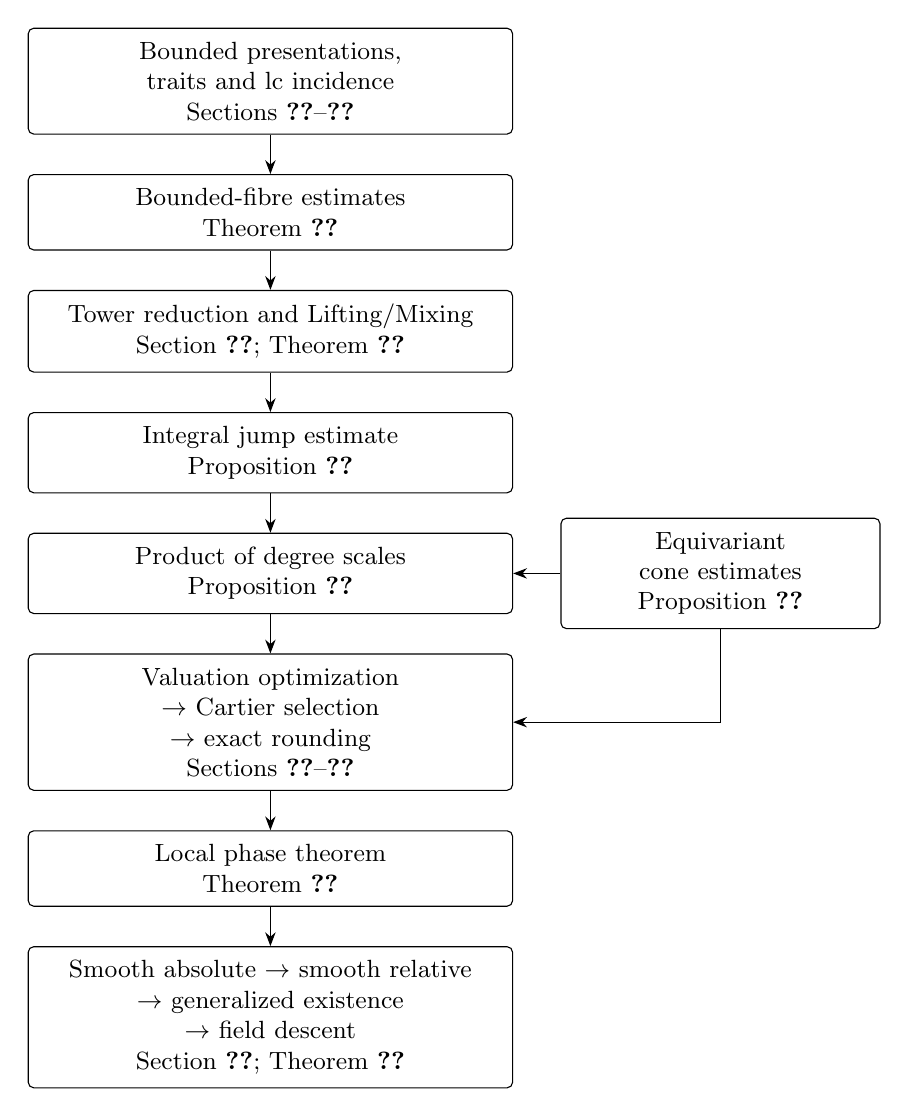
\begin{tikzpicture}[
 box/.style={draw,rounded corners=2pt,align=center,text width=5.8cm,
 minimum height=0.8cm,inner sep=5pt,font=\small},
 side/.style={box,text width=3.7cm},
 >={Stealth[length=5pt]},node distance=0.5cm and 0.6cm]
 \node[box] (prepare) {Bounded presentations, traits and lc incidence\\Sections~\ref{sec:bounded-presentations}--\ref{sec:incidence}};
 \node[box,below=of prepare] (bounded) {Bounded-fibre estimates\\Theorem~\ref{thm:bounded-fibre}};
 \node[box,below=of bounded] (tower) {Tower reduction and Lifting/Mixing\\Section~\ref{sec:tower}; Theorem~\ref{thm:lifting-mixing}};
 \node[box,below=of tower] (jump) {Integral jump estimate\\Proposition~\ref{prop:integral-jump}};
 \node[box,below=of jump] (product) {Product of degree scales\\Proposition~\ref{prop:product}};
 \node[side,right=of product] (cone) {Equivariant cone estimates\\Proposition~\ref{prop:cone-estimates}};
 \node[box,below=of product] (select) {Valuation optimization\\$\to$ Cartier selection\\$\to$ exact rounding\\Sections~\ref{sec:valuative}--\ref{sec:rounding}};
 \node[box,below=of select] (phase) {Local phase theorem\\Theorem~\ref{thm:phase}};
 \node[box,below=of phase] (global) {Smooth absolute $\to$ smooth relative\\$\to$ generalized existence\\$\to$ field descent\\Section~\ref{sec:global}; Theorem~\ref{thm:main}};
 \foreach \a/\b in {prepare/bounded,bounded/tower,tower/jump,jump/product,product/select,select/phase,phase/global}
   \draw[->] (\a)--(\b);
 \draw[->] (cone)--(product);
 \draw[->] (cone.south) |- (select.east);
\end{tikzpicture}
\end{document}
